\documentclass[11pt,a4j]{jarticle}
%\usepackage{psfig}
\usepackage[dvipdfmx]{graphicx} % use \includegrahpics
\def\figref#1{図~\ref{#1}}
\def\tabref#1{表~\ref{#1}}
%\def\eqref#1{\ref{#1}~式}
\def\secref#1{\ref{#1}~節}


%%============================================================
%% Layout
%% = = = = = = = = = = = = = = = = = = = = = = = = = = = = = =

\def\setmargin#1#2#3{%	side/top/bottom
	\textwidth = 210mm	%%% Full Size
	\textheight = 296mm	%%% Full Size
	\topmargin = -38mm	%%% 0mm
	\oddsidemargin = -26mm	%%% 0mm
%
	\advance\oddsidemargin + #1
	\evensidemargin = \oddsidemargin
	\advance\textwidth - #1	
	\advance\textwidth - #1
%
	\advance\topmargin + #2
	\advance\textheight - #2 
	\advance\textheight - #3
}

\setmargin{20mm}{25mm}{25mm}


%%----------------------------------------------------------------------
%%
\usepackage{bm}
\usepackage{amsmath}
\usepackage{amssymb}
\usepackage{amsfonts}\def\argmax{\operatorname*{argmax}}


%\def\V#1{\mbox{\boldmath $#1$}}
%\def\M#1{\mbox{\boldmath $#1$}}
%\def\S#1{\mbox{\boldmath $#1$}}
%\def\Ts#1{\mbox{\boldmath $#1$}}
\def\V#1{{\bm{#1}}}  % ベクトル
\def\M#1{{\bm{#1} }} % 行列
\def\Ts#1{{\bm{#1}}} % テンソル
\def\S#1{{\mathbb{#1}}}  % 集合

\def\Va#1{{\overrightarrow{#1}}} % 矢印ベクトル

\def\MtxK#1#2{\left[ \begin{array}[c]{#1} #2 \end{array} \right]}
\def\Vec#1{\MtxK{c}{#1}}
\def\Mtxxxx#1{\MtxK{cccc}{#1}}
\def\Mtxx#1{\MtxK{cc}{#1}}
\def\Mtx#1{\MtxK{c}{#1}}
\def\Tsr#1{\MtxK{c}{#1}}

\def\Seq#1{\left\{ #1 \right\}}
\def\Set#1{\left\{ #1 \right\}}
\def\Tuple#1{\left< #1 \right>}

% 転置
%\def\Tr#1{{}^{\mathrm{T}}{#1}}
\def\Tr#1{{}^{\top}\!{#1}}

%%----------------------------------------------------------------------
\def\Deg#1{^{\left< #1 \right>}}  % 次数
\def\Cxc#1{{#1}^{\dagger}} % 複素共役

\def\Abs#1{\left| #1 \right|}


\def\Dpd{\times} %% 直積記号 : direct product
\def\Kpd{\otimes} %% クロネッカー積記号 : Kronecker product
\def\Apd{\circ} %% アダマール積記号 : Kronecker product
\def\DpA#1{\bar{#1}}  %% 直積の値の頭につけるアクセント

\def\Ipd{\cdot}  %% 内積
\def\Opd{\times} %% 外積

\def\MxA#1{\hat{#1}}  %%  混合分布につけるアクセント

%%----------------------------------------------------------------------
\def\Opt#1{{#1}^{*}}    %% optimum
\def\Est#1{\hat{#1}}    %% estimate
\def\Apx#1{\tilde{#1}}  %% approx
%\def\Tch#1{#1^{*}}       %% teacher
\def\Tch#1{\overset{\circ}{#1}}       %% teacher

\def\Tm#1{^{\left< #1 \right>}}  % 回数

\def\Ly#1{\langle #1 \rangle}  %% layer
\def\In{_{\text{\sc in}}{}}

%%----------------------------------------------------------------------
\def\Orth{\bot}  %% 垂直
%\def\Para{\parallel}  %% 平行。欧米式。
\def\Para{{\mathbin{\!/\mkern-5mu/\!}}}  %% 平行。日本式。

%%----------------------------------------------------------------------
\def\Av#1{\left|#1\right|}
\def\SD#1{\sigma_{#1}}
\def\Var#1{\SD{#1}^2}
\def\Avg#1{\mu_{#1}}
\def\Xpt#1{\bar{#1}}  %% 期待値



\makeatletter
  \def\@LkS{{\cal L}}    %% likelihood Symbol
  \def\@LkF[#1]{\@LkS\left(#1\right)}    %% likelihood func.
  \def\Lk{\@ifnextchar[{\@LkF}{\@LkS}% ]
         }
\makeatother

\makeatletter
  \def\@PrSym{{\cal P}}
  \def\Pr{\@ifnextchar[{\@Pr}{\@PrSym}% ]
  }
  \def\@Pr[#1]{\@PrSym\left(#1\right)}

  %% Gaussian  G[x;\mu,\sigma]
  \def\@GSym{{\cal G}}        
  \def\G{\@ifnextchar[{\@G}{\@GSym}% ]
  }
  \def\@G[#1]{\@GSym\left(#1\right)}

%% 二項分布・Binomial 
  \def\@BnSym{{\cal B}}
  \def\Bn{\@ifnextchar[{\@Bn}{\@BnSym}% ]
  }
  \def\@Bn[#1]{\@BnSym\left(#1\right)}

%% 幾何分布・geometric distribution
  \def\@GmSym{\mathsf{g}}
  \def\Gm{\@ifnextchar[{\@Gm}{\@GmSym}% ]
  }
  \def\@Gm[#1]{\@GmSym\left(#1\right)}

%% noise
  \def\nz{\epsilon}	

  \def\@KLDivSym{\mathfrak{D}_{_{\mathsf{KL}}}}
  \def\KLDiv#1{\def\@@foo{#1}\@KLDivSym\ifx\@@foo\empty {} \else \left[ #1 \right] \fi}

%  \def\@LossFuncSym{\mathfrak{L}}
  \def\@LossFuncSym{\mathcal{L}}
  \def\LossFunc#1{\def\@@foo{#1}\@LossFuncSym\ifx\@@foo\empty {} \else \left[ #1 \right] \fi}

\makeatother


\def\EqDesc#1{\mbox{\ \ \ ; #1}}


\makeatletter
\def\Lp{\@ifnextchar[{\@Lp}{{\cal L}}} %% ラプラス変換 \Lp[f] or \Lp(f)
\def\@Lp[#1]{\Lp{}\left[#1\right]}
\def\ILp{\@ifnextchar[{\@ILp}{{\cal L}^{-1}}} %% ラプラス変換 \Lp[f] or \Lp(f)
\def\@ILp[#1]{\ILp{}\left[#1\right]}
\makeatother

\def\Conv{\ast}  %% 畳み込み積分 (Convolution Integral)
\def\Comb#1#2{{}_{#1}C_{#2}}

%%----------------------------------------------------------------------
\def\argmin{\operatorname*{argmin}}
\def\argmax{\operatorname*{argmax}}
\def\Linear{\operatorname{linear}}
\def\StepFunc{\operatorname{step}}
\def\SignFunc{\operatorname{sign}}
\def\Sigmoid{\operatorname{sigmoid}}
\def\VSigmoid{\mathbf{sigmoid}}
\def\BSigmoid{\operatorname{bi\_sigmoid}}
\def\ErrorFunc{\operatorname{erf}}
\def\ReLU{\operatorname{ReLU}}
\def\Softplus{\operatorname{softplus}}
\def\Softmax{\operatorname{softmax}}
\def\Attention{\operatorname{Attention}}

%%======================================================================

\def\Where{\mbox{\hspace{3em}} ; \mbox{\hspace{1em}}}
\def\where0pt{\makebox[0pt][l]{\mbox{where}} \nonumber}


\def\MyBox#1{{\unitlength=#1 \framebox(1,1){}}}
\def\MyFillBox#1{\rule{#1}{#1}}
\def\EOTH{\hfill\MyBox{.5em}}
\def\QED{\hfill\MyFillBox{.5em}}

\newenvironment{Note}[1]{%
%  \paragraph*{ノート: #1} \fill \rule{0.5\textwidth}{1pt}
  \paragraph{\protect\MyFillBox{1em} ノート--- #1} \hrule%
  \hfill 
}{%
  \hfill\MyBox{1em}\hrule
  \ \\
}

%%======================================================================

\newif\ifWideBoxedEqnarray
\WideBoxedEqnarraytrue
\WideBoxedEqnarrayfalse

\newenvironment{BoxedEqnarray}{%
  \vspace{-4ex}
  \begin{center}%
    \begin{tabular}[c]{|c|} \hline%
      \begin{minipage}[c]{\textwidth}  %{width}
      \ifWideBoxedEqnarray%
        \vspace{-0.5ex} %
      \else%
        \vspace{-2.3ex} %
      \fi%
        \begin{eqnarray}%
}{%
        \end{eqnarray}%
      \end{minipage}%
      \ifWideBoxedEqnarray%
        \\%
      \else%
        % nothing
      \fi%
%      \\
      \\ \hline%
    \end{tabular}
  \end{center}%
}

%%======================================================================

\def\DefPrefix{定義}
\def\LemmaPrefix{補題}
\def\TheoremPrefix{定理}
\newtheorem{genericTheorems}{GenericTheorem}[section]
\newtheorem{xDef}[genericTheorems]{\DefPrefix}
\newtheorem{xLemma}[genericTheorems]{\LemmaPrefix}
\newtheorem{xTheorem}[genericTheorems]{\TheoremPrefix}

\newenvironment{Lemma}{%
  \begin{xLemma}%
    \addcontentsline{toc}{subparagraph}{%
      \fbox{\LemmaPrefix \thexLemma}}
  \ \\
}{%
  \EOTH%
  \end{xLemma}%
}

\newenvironment{Theorem}{%
  \begin{xTheorem}%
    \addcontentsline{toc}{subparagraph}{%
      \fbox{\TheoremPrefix \thexLemma}}
  \ \\
}{%
  \EOTH
  \end{xTheorem}%
}


%%======================================================================
% 数式中のコメントのためのタブ
\def\ComTab{\mbox{\;\; ; \;\;}}



\iftrue
%\iffalse
\includeonly{
%  ch010_complexGauss
  ch020_entangle
  }
\fi

%\def\ClearPage{\clearpage}
\def\ClearPage{\cleardoublepage}


\begin{document}
%%----------------------------------------------------------------------
\title{Itk::Geo3D Notes}
\author{野田 五十樹}
\date{%
  {\scriptsize
  \begin{tabular}[c]{|l|l|} \hline
  2024/10/04 & 初期バージョン \\ \hline
  2024/10/20 & 屈曲点での円周接続 \\ \hline
 \end{tabular}
  }
}
\maketitle
%% - - - - - - - - - - - - - - - - - - - - - - - - - - - - - - - - - - -
\setcounter{tocdepth}{10}

%\iftrue
\iffalse
\ClearPage
\tableofcontents
\ClearPage\cleardoublepage
\fi
%% - - - - - - - - - - - - - - - - - - - - - - - - - - - - - - - - - - -



%%----------------------------------------------------------------------
\section{class LineSegment}
%% - - - - - - - - - - - - - - - - - - - - - - - - - - - - - - - - - - -

%%--------------------------------------------------
\subsection{closestFractionPairFrom()}
%% - - - - - - - - - - - - - - - - - - - - - - - - -
3次元(以上)の2つの線分の最近点を求める。
求めるものは、各線分上の分率とする。

%%>>>>>>>>>>>>>>>>>>>>>>>>>>>>>>>>>>>>>>>>>>>>>>>>>>
\begin{figure}[h]
  \centering
  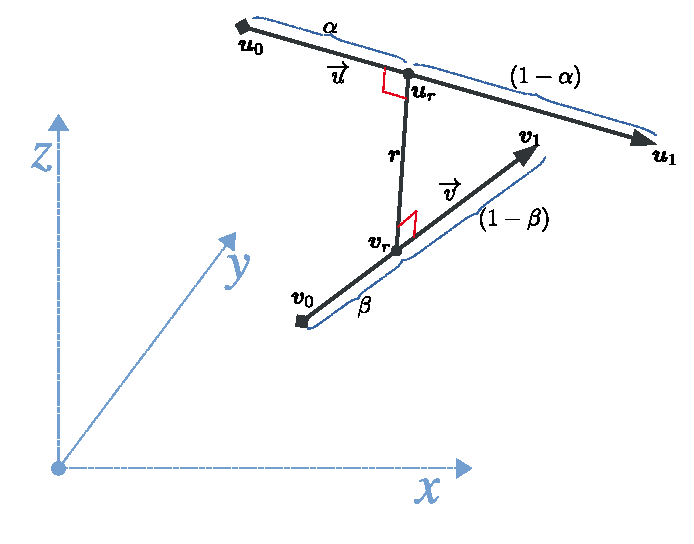
\includegraphics[width=.5\linewidth]{Fig/figure-01.eps}
  \caption{2つの線分の最近距離}
  \label{fig:Fig/figure-01.eps}
\end{figure}
%%>>>>>>>>>>>>>>>>>>>>>>>>>>>>>>>>>>>>>>>>>>>>>>>>>>

まず、2つの線分 $\V{u},\V{v}$ を考える(\figref{fig:Fig/figure-01.eps})。
  %%$$$$$$$$$$$$$$$$$$$$$$$$$$$$$$$$$$$$$$$$
  \begin{eqnarray}
    \V{u} & = & \Tuple{\V{u}_0, \V{u}_1}
  \\
    \V{v} & = & \Tuple{\V{v}_0, \V{v}_1}
  \end{eqnarray}
  %%$$$$$$$$$$$$$$$$$$$$$$$$$$$$$$$$$$$$$$$$
ただし、$ \Tuple{\V{u}_0, \V{u}_1} $ は、
位置 $\V{u}_0$ から位置 $\V{u}_1$ から位置への線分を表す。

線分 $\V{u},\V{v}$ 上の任意の点 $\V{u}_r,\V{u}_r$ は、
その分率を各々 $\alpha,\beta$ として、
次のように表される。
  %%$$$$$$$$$$$$$$$$$$$$$$$$$$$$$$$$$$$$$$$$
  \begin{eqnarray}
    \V{u}_r & = & (1-\alpha) \V{u}_0 + \alpha \V{u}_1
  \\
    \V{v}_r & = & (1-\beta)  \V{v}_0 + \beta  \V{v}_1
  \end{eqnarray}
  %%$$$$$$$$$$$$$$$$$$$$$$$$$$$$$$$$$$$$$$$$
ここで、$\V{r}_u,\V{r}_v$を両端とする線分 $\V{r}$ を考える。
  %%$$$$$$$$$$$$$$$$$$$$$$$$$$$$$$$$$$$$$$$$
  \begin{eqnarray}
    \V{r} & = & \Tuple{\V{u}_r,\V{u}_v}
  \end{eqnarray}
  %%$$$$$$$$$$$$$$$$$$$$$$$$$$$$$$$$$$$$$$$$
また、この線分の方向 $\V{r}_d$ は
  %%$$$$$$$$$$$$$$$$$$$$$$$$$$$$$$$$$$$$$$$$
  \begin{eqnarray}
    \V{r}_d
      & = & \V{v}_r - \V{u}_r
  \\
      & = &
        - \alpha (\V{u}_1 - \V{u}_0)
        + \beta  (\V{v}_1 - \V{v}_0)
        + (\V{v}_0 - \V{u}_0)
  \end{eqnarray}
  %%$$$$$$$$$$$$$$$$$$$$$$$$$$$$$$$$$$$$$$$$

線分 $\V{r}$ が $\V{u},\V{v}$ の最近点を結ぶ線分とすると、
直線 $\V{r}$ と2つの直線 $\V{u},\V{v}$ は互いに直交する。
	\footnote{本来、線分は両端をはみ出さないが、ここでは話を簡単にするため、
	  直線で考える。}
よって、以下の等式が成立する。
  %%$$$$$$$$$$$$$$$$$$$$$$$$$$$$$$$$$$$$$$$$
  \begin{eqnarray}
    (\V{v}_r - \V{u}_r) (\V{u}_1 - \V{u}_0) & = & 0
  \\
    (\V{v}_r - \V{u}_r) (\V{v}_1 - \V{v}_0) & = & 0
  \end{eqnarray}
  %%$$$$$$$$$$$$$$$$$$$$$$$$$$$$$$$$$$$$$$$$
すなわち、
  %%$$$$$$$$$$$$$$$$$$$$$$$$$$$$$$$$$$$$$$$$
  \begin{eqnarray}
    - \alpha (\V{u}_1 - \V{u}_0)^2
    + \beta  (\V{u}_1 - \V{u}_0)(\V{v}_1 - \V{v}_0)
    + (\V{v}_0 - \V{u}_0)(\V{u}_1 - \V{u}_0)
      & = & 0
  \label{eq:r*u}
  \\
    - \alpha (\V{u}_1 - \V{u}_0)(\V{v}_1 - \V{v}_0)
    + \beta  (\V{v}_1 - \V{v}_0)^2
    + (\V{v}_0 - \V{u}_0)(\V{v}_1 - \V{v}_0)
      & = & 0
  \label{eq:r*v}
  \end{eqnarray}
  %%$$$$$$$$$$$$$$$$$$$$$$$$$$$$$$$$$$$$$$$$
ここで、以下の置き換えを行う。
  %%$$$$$$$$$$$$$$$$$$$$$$$$$$$$$$$$$$$$$$$$
  \begin{eqnarray}
    a & = & (\V{u}_1 - \V{u}_0)^2
  \\
    b & = & (\V{v}_1 - \V{v}_0)^2
  \\
    c & = & (\V{u}_1 - \V{u}_0) (\V{v}_1 - \V{v}_0)
  \\
    g & = & (\V{v}_0 - \V{u}_0) (\V{u}_1 - \V{u}_0)
  \\
    h & = & (\V{v}_0 - \V{u}_0) (\V{v}_1 - \V{v}_0)
  \end{eqnarray}
  %%$$$$$$$$$$$$$$$$$$$$$$$$$$$$$$$$$$$$$$$$
これにより、\eqref{eq:r*u},\eqref{eq:r*v}は以下のベクトル式で書ける。
  %%$$$$$$$$$$$$$$$$$$$$$$$$$$$$$$$$$$$$$$$$
  \begin{eqnarray}
    \Mtxx{-a & c \\ -c & b} \Vec{\alpha \\ \beta}
      & = &
        \Vec{-g \\ -h}
  \end{eqnarray}
  %%$$$$$$$$$$$$$$$$$$$$$$$$$$$$$$$$$$$$$$$$
  %%$$$$$$$$$$$$$$$$$$$$$$$$$$$$$$$$$$$$$$$$
  \begin{eqnarray}
    \Vec{\alpha \\ \beta}
      & = &
        \Mtxx{-a & c \\ -c & b}^{-1} 
        \Vec{-g \\ -h}
  \\
      & = &
        \frac{-1}{\det}
        \Mtxx{b & -c \\ c & -a}
        \Vec{g \\ h}
  \end{eqnarray}
  %%$$$$$$$$$$$$$$$$$$$$$$$$$$$$$$$$$$$$$$$$
ただし、$\det$ は上記行列の行列式の値であり、以下の通り。
  %%$$$$$$$$$$$$$$$$$$$$$$$$$$$$$$$$$$$$$$$$
  \begin{eqnarray}
    \det
      & = &
        c^2 - ab
  \end{eqnarray}
  %%$$$$$$$$$$$$$$$$$$$$$$$$$$$$$$$$$$$$$$$$

ここで求まった $\alpha, \beta$ が区間 $[0,1]$ の間であれば、
頂点 $\V{u}_r, \V{v}_r$ は各々、線分 $\V{u}, \V{v}$ 上にある。
それ以外の場合は、直前 $\V{u}, \V{v}$ 上となる。

一方、行列式の値 $\det$ が 0 となるのは、
  %%$$$$$$$$$$$$$$$$$$$$$$$$$$$$$$$$$$$$$$$$
  \begin{eqnarray}
    c^2 - ab
      & = &
        ((\V{u}_1 - \V{u}_0) (\V{v}_1 - \V{v}_0))^2 -
        (\V{u}_1 - \V{u}_0)^2 (\V{v}_1 - \V{v}_0)^2
      = 0
  \\
    ((\V{u}_1 - \V{u}_0) (\V{v}_1 - \V{v}_0))^2
      & = &
        (\V{u}_1 - \V{u}_0)^2 (\V{v}_1 - \V{v}_0)^2
  \\
    (\V{u}_1 - \V{u}_0) (\V{v}_1 - \V{v}_0)
      & = &
        \Abs{\V{u}_1 - \V{u}_0} \Abs{\V{v}_1 - \V{v}_0}
  \end{eqnarray}
  %%$$$$$$$$$$$$$$$$$$$$$$$$$$$$$$$$$$$$$$$$
これは、線分 $\V{u}, \V{v}$ が並行の場合である。
この場合は、$\alpha = \beta = 0$ としてよい。
\footnote{正確には、線分の方向により一方を 1 にする必要がある。}



%%----------------------------------------------------------------------
\section{class Triangle}
%% - - - - - - - - - - - - - - - - - - - - - - - - - - - - - - - - - - -

%%--------------------------------------------------
\subsection{orthogonalDirection()}
%% - - - - - - - - - - - - - - - - - - - - - - - - -
3次元(以上)の空間にある3点 $\V{p}, \V{q}, \V{r}$ で定まる平面$S$の方向 $\V{s}$ を
考える。
ただし、平面$S$の方向とは、平面に対して垂直な方向とする。
また、その平面$S$は原点 $[0,0,0]$ を含まないものとする。
  \footnote{原点を含む場合は、座標系全体を平行移動して原点を含まないようにする。}

%%>>>>>>>>>>>>>>>>>>>>>>>>>>>>>>>>>>>>>>>>>>>>>>>>>>
\begin{figure}[h]
  \centering
  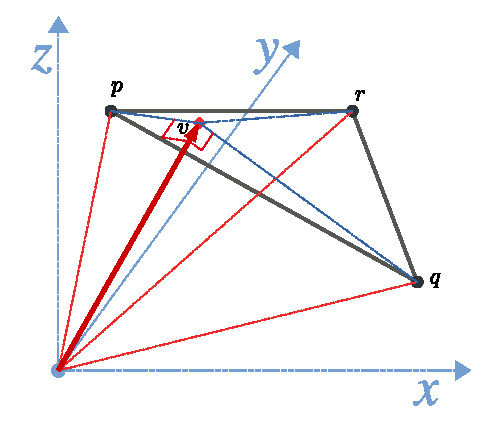
\includegraphics[width=.5\linewidth]{Fig/figure-02.eps}
  \caption{三角形と垂線(法線)}
  \label{fig:Fig/figure-02.eps}
\end{figure}
%%>>>>>>>>>>>>>>>>>>>>>>>>>>>>>>>>>>>>>>>>>>>>>>>>>>

  
平面 $S$ 上の点 $\V{v}$は以下の式で表される。
  %%$$$$$$$$$$$$$$$$$$$$$$$$$$$$$$$$$$$$$$$$
  \begin{eqnarray}
    \V{v}
      & = &
        \alpha \V{p} + \beta \V{q} + (1-\alpha-\beta)\V{r}
  \end{eqnarray}
  %%$$$$$$$$$$$$$$$$$$$$$$$$$$$$$$$$$$$$$$$$
ただし、$\alpha, \beta$ は実数とする。
なお、$\alpha, \beta$ が以下の範囲の時、
$\V{v}$ は三角形 $\Tuple{\V{p},\V{q},\V{r}}$ の内部にある。
  %%$$$$$$$$$$$$$$$$$$$$$$$$$$$$$$$$$$$$$$$$
  \begin{eqnarray}
    & 0 < \alpha < 1
  \\
    & 0 < \beta < 1
  \\
    & 0 < (1-\alpha-\beta) < 1
  \end{eqnarray}
  %%$$$$$$$$$$$$$$$$$$$$$$$$$$$$$$$$$$$$$$$$

ここで、ベクトル $\V{v}$ が平面 $S$ に垂直であるとする。
この場合、以下が成立する。
  %%$$$$$$$$$$$$$$$$$$$$$$$$$$$$$$$$$$$$$$$$
  \begin{eqnarray}
    \V{v} (\V{p} - \V{r}) & = & 0
  \\
    \V{v} (\V{q} - \V{r}) & = & 0
  \end{eqnarray}
  %%$$$$$$$$$$$$$$$$$$$$$$$$$$$$$$$$$$$$$$$$
つまり、
  %%$$$$$$$$$$$$$$$$$$$$$$$$$$$$$$$$$$$$$$$$
  \begin{eqnarray}
      \alpha (\V{p} - \V{r})^2
    + \beta  (\V{q} - \V{r}) (\V{p} - \V{r})
    + \V{r} (\V{p} - \V{r})
      & = & 0
  \label{eq:alpha-qr-beta-qrpr}
  \\
      \alpha (\V{p} - \V{r}) (\V{q} - \V{r})
    + \beta  (\V{p} - \V{r})^2
    + \V{r} (\V{q} - \V{r})
      & = & 0
  \label{eq:alpha-prqr-beta-qr}
  \end{eqnarray}
  %%$$$$$$$$$$$$$$$$$$$$$$$$$$$$$$$$$$$$$$$$
ここで以下の置き換えを行う。
  %%$$$$$$$$$$$$$$$$$$$$$$$$$$$$$$$$$$$$$$$$
  \begin{eqnarray}
    a & = & (\V{p} - \V{r})^2
  \\
    b & = & (\V{p} - \V{r}) (\V{q} - \V{r})
  \\
    c & = & (\V{q} - \V{r})^2
  \\
    g & = & \V{r} (\V{p} - \V{r})
  \\
    h & = & \V{r} (\V{q} - \V{r})
  \end{eqnarray}
  %%$$$$$$$$$$$$$$$$$$$$$$$$$$$$$$$$$$$$$$$$
これにより、\eqref{eq:alpha-qr-beta-qrpr}、\eqref{eq:alpha-prqr-beta-qr}は
以下のように表記できる。
  %%$$$$$$$$$$$$$$$$$$$$$$$$$$$$$$$$$$$$$$$$
  \begin{eqnarray}
    \Mtxx{a & b \\ b & c} \Vec{\alpha \\ \beta}
      & = &
        -\Vec{g \\ h}
  \end{eqnarray}
  %%$$$$$$$$$$$$$$$$$$$$$$$$$$$$$$$$$$$$$$$$
よって、$\alpha, \beta$ は以下の式で求まる。
  %%$$$$$$$$$$$$$$$$$$$$$$$$$$$$$$$$$$$$$$$$
  \begin{eqnarray}
    \Vec{\alpha \\ \beta}
      & = &
        \Mtxx{a & b \\ b & c}^{-1} 
        \left( -\Vec{g \\ h} \right)
  \\
      & = &
        \frac{-1}{\det} \Mtxx{c & -b \\ -b & a}
        \Vec{g \\ h}
  \\
    \det
      & = &
        ac - b^2
  \end{eqnarray}
  %%$$$$$$$$$$$$$$$$$$$$$$$$$$$$$$$$$$$$$$$$
なお、 $\det = 0$ では上記解は求まらない。
これは、$\V{p},\V{q},\V{r}$ の3点の内2つが一致している場合である。


%%--------------------------------------------------
\subsection{orthogonalDirection2()}
%% - - - - - - - - - - - - - - - - - - - - - - - - -
外積の定義より推薦を計算する。

2つのベクトル $\V{u}, \V{v}$ について、以下のような外積 $\V{w}$は、
以下の性質を満たす。
  %%$$$$$$$$$$$$$$$$$$$$$$$$$$$$$$$$$$$$$$$$
  \begin{eqnarray}
    \V{w}
      & = &
        \V{u} \Opd \V{v}
  \\
      & = &
        \Vec{u_y v_z - u_z v_y \\
             u_z v_x - u_x v_z \\
             u_x v_y - u_y v_z}
  \\
    \V{w} \Ipd \V{u}
      & = &
        0
  \\
    \V{w} \Ipd \V{v}
      & = &
        0
  \\
    \Abs{\V{w}}
      & = &
        \mbox{$\V{u}$, $\V{v}$ が張る三角形の面積}
  \end{eqnarray}
  %%$$$$$$$$$$$$$$$$$$$$$$$$$$$$$$$$$$$$$$$$

%%>>>>>>>>>>>>>>>>>>>>>>>>>>>>>>>>>>>>>>>>>>>>>>>>>>
\begin{figure}[h]
  \centering
  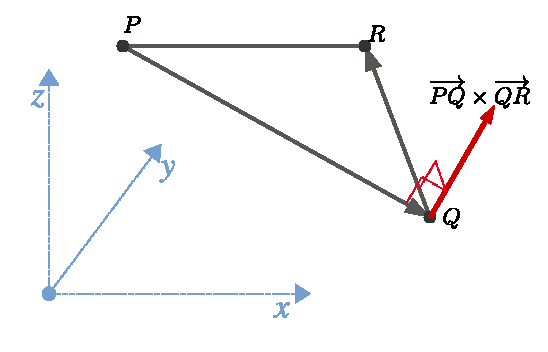
\includegraphics[width=.5\linewidth]{Fig/figure-03.eps}
  \caption{三角形と外積による垂線(法線)}
  \label{fig:Fig/figure-03.eps}
\end{figure}
%%>>>>>>>>>>>>>>>>>>>>>>>>>>>>>>>>>>>>>>>>>>>>>>>>>>

このベクトルの外積を使って、
\figref{fig:Fig/figure-03.eps} のような
三角形 $PQR$ に対する垂線$\V{h}$ は以下のように求めることができる。
 
  %%$$$$$$$$$$$$$$$$$$$$$$$$$$$$$$$$$$$$$$$$
  \begin{eqnarray}
    P: \V{p}
      & = &
        \Tr{\Vec{p_x, p_y, p_z}}
  \\
    Q: \V{q}
      & = &
        \Tr{\Vec{q_x, q_y, q_z}}
  \\
    R: \V{r}
      & = &
        \Tr{\Vec{r_x, r_y, r_z}}
  \end{eqnarray}
  %%$$$$$$$$$$$$$$$$$$$$$$$$$$$$$$$$$$$$$$$$
  \begin{eqnarray}
    \Va{PQ}
      & = &
        \Tr{\Vec{q_x - p_x, q_y - p_y, q_z - p_z}}
  \\
    \Va{QR}
      & = &
        \Tr{\Vec{r_x - q_x, r_y - q_y, r_z - q_z}}
  \end{eqnarray}
  %%$$$$$$$$$$$$$$$$$$$$$$$$$$$$$$$$$$$$$$$$
  \begin{eqnarray}
    \V{h}
      & = &
        \Va{PQ} \Opd \Va{QR}
  \\
      & = &
        \Vec{(q_y - p_y)(r_z - q_z) - (q_z - p_z)(r_y - q_y) \\
             (q_z - p_z)(r_x - q_x) - (q_x - p_x)(r_z - q_z) \\
             (p_x - p_x)(r_y - q_y) - (q_y - p_y)(r_x - q_x)}
  \end{eqnarray}
  %%$$$$$$$$$$$$$$$$$$$$$$$$$$$$$$$$$$$$$$$$

%%--------------------------------------------------
\subsection{屈曲点での半径 $R$ の接続とセットバック}
%% - - - - - - - - - - - - - - - - - - - - - - - - -

%%>>>>>>>>>>>>>>>>>>>>>>>>>>>>>>>>>>>>>>>>>>>>>>>>>>
\begin{figure}[h]
  \centering
  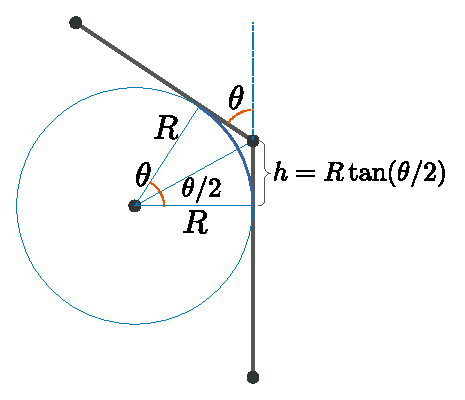
\includegraphics[width=.6\linewidth]{Fig/figure-04.eps}
  \caption{屈曲点での円周に寄る接続とセットバック}
  \label{fig:Fig/figure-04.eps}
\end{figure}
%%>>>>>>>>>>>>>>>>>>>>>>>>>>>>>>>>>>>>>>>>>>>>>>>>>>


2つの連続する線分が角度 $\theta$ をつけて曲がっている時、
その屈曲点で半径 $R$ の円周で接続することを考える。
この場合、円周と線分の接点と屈曲点の間の距離(セットバック)を $h$ とする
(\figref{fig:Fig/figure-04.eps})。

この $h$ は以下の式で表すことができる。
  %%$$$$$$$$$$$$$$$$$$$$$$$$$$$$$$$$$$$$$$$$
  \begin{eqnarray}
    h
      & = &
        R \tan \frac{\theta}{2}
  \end{eqnarray}
  %%$$$$$$$$$$$$$$$$$$$$$$$$$$$$$$$$$$$$$$$$



  
\end{document}
